
\begin{abstract}
Pulsars are excellent testing grounds for fundamental physics. As precise
cosmic clocks, they have been used in many experiments, especially in testing
gravitational theories. We report 20-year timing of one of the most precise
pulsar---J1713+0747. The results can be used to constrain alternative
gravitational theories and test the constancy of the gravitational constant.
\end{abstract}


\section{Introduction}
We present 20-year timing of the millisecond  PSR J1713+0747. Discovered in
1993 \citep{fwc93}, PSR J1713+0747 is one of the brightest pulsars timed by the
North American nano-Hertz Observatory for Gravitation Waves (NANOGrav;
\citealt{ndf+12, dfg+13}). It also has the smallest timing residual of all NANOGrav pulsars \citep{dfg+13}. Observed with the largest telescope in the world, the Arecibo Observatory, it is probably one of the most well-timed pulsar in the world.

The high timing precision and the long base line allowed us to measure precisely
the pulsar binary system's  masses, orbit, distance, proper motion, and even
the orientation of the orbit on the sky. More importantly, 
we measured the binary orbital period to very high precision, and detected a
very small orbital decay over the 20 years time span. This allow us to test
Einstein's theory of Gravity as well as some alternative theories.


The Jordan-Fierz-Brans-Dicke theory \citep{jor59,fie56,bd61} describes a class of alternative theories of Gravity. 
This class of theories modifies Einstein's equation of dynamics by coupling
mass with a scalar-tensor
field. Therefore, it is also referred to as the scalar-tensor gravity. 
This is one of the last alternative theories of Gravity that is still not
ruled out, although, fairly stringent constrain have been placed on the coupling
strength of the scalar field based on observations of binary systems
\citep{hmb10, lwj+09, fwe+12}.


\section{Observations}
Timing observation of PSR J1713+0747 started from 1993 at the Arecibo
Observatory. \citet{sns+05} reported the first 12 years timing result. After
that, J1713+0747 was monitored regularly as part of  NANOGrav's pulsar timing
array project. It is observed monthly in L band and S band by the Arecibo Observatory and in 800MHz and L band by the Green Bank Observatory.

\section{Timing model}
\label{timing_model}
A comprehensive timing model was described by \citet{sns+05}, this model includes the effect of pulsar rotation, astrometry, orbital motion, Shapiro delay and dispersion effect due to interstellar median.
We employed the same \citet{dd86} model they used to fit for the pulsar and its orbital motions, we also used the DMX model to fit DM changes (see Section \ref{sec:dmx} for detail), and we used an improved model to deal with profile evolution in frequency (see Section \ref{sec:pfev} for detail). 
In the pulsar model, we added an extra fitting parameter, the change rate of binary period $\dot{P}_{\rm b}$ to model a previously undetectable change in $P_{\rm b}$.This is described in Section \ref{sec:obdecay}.    
We can confirm that most of the pulsar-binary parameters that \citet{sns+05} got still works for the 20 years data. The new timing model parameters (Table \ref{tab:par}) differs from the \citet{sns+05} slightly but consistent with their reported uncertainties.


\subsection{DM variation}
\label{sec:dmx}
The DM of a pulsar characterizes how much interstellar median (ISM) lies
between the pulsar and us, and it changes as the ISM varies. For most pulsar
this change is too small to be detectable. However, for pulsars with residual
$\lesssim1\mu$s, the contribution from varying ISM start to contribute
significantly to the timing noise. 

Using the {\it DMX} model in {\it tempo}, we were able to fit for DM
variation. 
The model groups TOA from observations taken within ten days and fit for the
best DM for each group.   
It was applied to TOA from Mark4, ABPP, ASP, GAPS, GUPPI, and PUPPI data, but
not for Mark3. Since Mark3 had only one frequency band (L-band), a precise DM
fitting was not possible from its data.
J1713+0747 was observed in L- and S-band by the Arecibo Observatory. The
two bands observations almost always happen one after another on the same day.
While GBT observes J1713+0747 in 800~MHz and L band but the two band
observations often are separated by less than ten days.
Therefore, most DM values in the {\it DMX} model was determined by TOA from at
least two bands. Figure \ref{fig:dmx} shows the DM variation of J1713+0747 
measured using the {\it DMX} model.
The pulsar shows a fractional DM changes of $\sim10^{-4}$.



\subsection{Pulse profile evolution in frequency}
\label{sec:pfev}
After removing the dispersion effect which corrects delays $\propto \nu^{-2}$
in the TOAs, small remaining frequency-dependent residuals were observed from
different instruments and telescopes (Figure \ref{fig:FD}).  
This phenomenon seems to be caused by the change of pulsar's pulse profile in
frequency, although the cause of such profile evolution is still unknown.
In \citet{sns+05}, a jump was fitted between even frequency channels in order to remove such effect, however, with the a factor of $\sim$10 increase of frequency channels from GUPPI, it would require many more jump parameters to be added to the timing model.
In light by the observation that the frequency-dependent-residual seems to
trace a smooth function, we used a rank-4 polynomial of the logarithm of
frequency to fit and removed this effect from the final residual ({\it FD}
model by P. Demorest et~al in prep.;see Figure \ref{fig:FD}). 



\subsection{Timing Noise and DM variation}

\subsubsection{Covariance with DM changes}
The lower band residuals are covariant with the DM changes.


\begin{itemize}
\item T2 model versus DD? confirms that both model gives pretty much consistent results?
\end{itemize}

\section{Result}

\subsection{Intrinsic orbital decay}
\label{sec:obdecay}
Through timing modeling, we measured a significant orbital decay from J1713+0747, $\dot{P}_{\rm b} = ?$. 
%Such a precise measurement can be used to test Gravitational wave radiation theories of Einstein's and beyond.
It is expected that the motion of the binary relate to the observer will introduce extra orbital decay due to kinetic effects, i.e. radial acceleration effect \citep{dt91} and centrifugal acceleration effect (`Shklovskii' effect; \citealt{shk70}). Luckily, we have good measurement on the distance and proper motion of the binary system, which allow us to remove these effects 
and study the system's intrinsic orbital decay.
\begin{equation}
\dot{P}_{\rm b}^{\rm Acc} = \frac{A_{\rm G}}{c} P_{\rm b} =
-1.2\pm0.1\times10^{-13}~{\rm s~s^{-1}}
\end{equation}
where $A_{\rm G}$ is the line-of-sight acceleration of the pulsar binary,
this term is dominated by the difference in the Galactic accelerations of the
binary and our solar system, and is obtained using
Equation 5 in \citet{nt95} and Equation 17 in \citet{lwj+09}.
\begin{equation}
\dot{P}_{\rm b}^{\rm Shk} = (\nu_{\alpha}^2+\nu_{\delta}^2)\frac{d}{c}P_{\rm
b} = 6.8\pm0.3\times10^{-13}~{\rm s~s^{-1}}
\end{equation}
Therefore, the pulsar's intrinsic orbital decay is $\dot{P}_{\rm b}^{\rm Int}
= \dot{P}_{\rm b}^{\rm Obs} - \dot{P}_{\rm b}^{\rm Shk} - \dot{P}_{\rm b}^{\rm
Gal} = (0.7\pm2)\times10^-13$s~s$^{-1}$, and is consistent with being smaller than measurable.

There are two extra classical terms that could have played a role in
$\dot{P}_{\rm b}^{\rm Int}$, one $\dot{P}_{\rm b}^{\dot{M}}$ is caused by mass loss in the
binary system, the other $ \dot{P}_{\rm b}^{\rm T}$ is the contribution of tidal effect.
The pulsar could loss mass due to its radiation, the maximum mass loss rate
due to this effect orbit can be estimated from its rotational energy loss rate
$\dot{M_{\rm psr}}<\dot{E}/c^2$, and similar idea may apply to the white
dwarf. 
%\begin{equation}
%\dot{P}_{\rm b}^{\dot{m}} = 8\pi^2\frac{I_{\rm
%PSR}}{Mc^2}\frac{\dot{P}}{P^3}P_{\rm b} \sim 10^{-16},
%\end{equation}
%where $M=M_{\rm PSR} +M_{\rm WD}$ is the total mass of the system and
%$I\sim10^{45}$g~cm$^2$ is the angular momentum of inertia.
Consequently, the orbital change due to mass loss is $\dot{P}_{\rm
b}^{\dot{M}}\lesssim 1\times10^{-14}$s~s$^{-1}$ (\citealt{dt91}; Equation 9 and 10
of \citealt{fwe+12}), an order of magnitude smaller than the measured
uncertainties on $\dot{P}_{\rm b}^{\rm Int}$.
The tidal effect of this binary system is expected to be $\dot{P}_{\rm b}^{\rm
T}\ll1\times10^{-14}$s~s$^{-1}$ basing on the most extreme scenarios (the WD spins at
its break-up velocity and the tidal synchronizing time scale equals the
characteristic age of the pulsar; see Equation 11 in \citealt{fwe+12} and
references therein in).
Both of these classical terms are much smaller than the observed uncertainties
on $\dot{P}_{\rm b}^{Int}$.
%The tidal effect can be estimated to $\sim$ according to Equation 11 of
%\citealt{fwe+12} and references therein. 


Finally, due to the 68 day orbit, the binary's  gravitational wave
radiation is so weak that its orbital decay according to Einstein's
theory is expected to be 
$\dot{P}_{\rm b}^{\rm GR} = -7\times10^{-18}$s~s$^{-1}$ \citep{lk05}.
This is consistent with the observed intrinsic orbital decay, therefore,
Einstein's theory of gravitational wave radiation pass this particular test.


\section{Constraint on $\dot{G}$}
\label{sec:Gdot}
Some alternative theories of gravity, such as the scalar-tensor gravity, predict extra orbital decay than Einstein's theory. 
Consequently, measurements of pulsar binaries' `excess' orbital decay
$\dot{P}_{\rm b}^{\rm exc}=\dot{P}_{\rm b}^{\rm Int} - \dot{P}_{\rm
b}^{\dot{M}}  - \dot{P}_{\rm b}^{\rm T} - \dot{P}_{\rm b}^{\rm GR}$ have been
used to constrain them \citep{lwj+09, fwe+12}. 
The measured values of $\dot{P}_{\rm b}^{\rm exc}$ from the pulsars of
previous work were all consistent with being zero. Their upper limits were largely determined by the uncertainties of $\dot{P}_{\rm b}^{\rm Int}$.
Thanks to the high time precision of NANOGrav observations, we measure the
orbital period of J1713+0747 to extreme high precision, which enable us to 
get $\dot{P}_{\rm b}^{\rm exc}=(0.7\pm2)\times10^-13$s~s$^{-1}$ (see Section
\ref{sec:obdecay} for detail). 
This is the smallest fractional orbital decay rate observed in pulsar binaries
due to J1713+0747's long orbit period, and can be used to put new limit on
the alternative theories of Gravity.

Extra orbital decay can be caused by the dipole gravitational radiation effect
introduced by some alternative gravity theories (\citealt{Will93, Will01, lwj+09, fwe+12} and reference therein). Such effect arise when the two bodies of binary are very different in terms of their self gravity, or in another word, their compactness.
This extra orbital decay is given by 
\begin{equation}
\dot{P}_{\rm b}^{\rm D} \simeq -4\pi\frac{T_{\odot}\nu}{P_{\rm b}}\kappa_D S^2,
\end{equation}
\citep{lwj+09}, where $T_{\odot}=G{\rm M_{\odot}}/c^3=4.9255$~${\rm \nu}$s, $\nu$ is the reduced mass $m_pm_c/M$ of the system , $\kappa_D $ is dipole
gravitational radiation "coupling constant", and $S$ is the difference
between the self-gravity "sensitivity" of the two bodies ($S = s_p - s_c$;
$s_p\sim0.1m_p/M_{\odot}$ according to \citealt{de92} ; and $s_c\ll s_p$).
In Einstein's GR $\kappa_D=0$ --- there is no self-gravity induced
dipole gravitational radiation, but it is often not the case in alternative
theories.

Another orbital decal term $\dot{P}_{\rm b}^{\dot{G}}$ is caused by a varying
local gravitational constant. In the framework of the scalar-tensor theories,
the scalar field that interacts with the mass has to change over time as the
Universe expands. This change will cause the locally measured gravitational
constant to vary. 
\begin{equation}
\dot{P}_{\rm b}^{\dot{G}} = -2 \frac{\dot{G}}{G}
\left[1-\left(1+\frac{m_c}{2M}\right)s_p\right]P_{\rm b}
\end{equation}
\citep{dgt88,nor90}.

The orbital period of J1713+0747 is relatively long among the
high-time-precision pulsar binaries, this make its $\dot{P}_{\rm b}^{\rm D}$
very small. Conversely, $\dot{P}_{\rm b}^{\dot{G}}$ is larger when $P_{\rm b}$
is large. This makes J1713+0747 the best pulsar binary system for constraining
the change rate of gravitational constant $\dot{G}$. A combined limit on both
$\dot{G}$ and the dipole gravitational radiation constant $\kappa_D$ can be
done in the same fashion as in \citet{lwj+09}: solving $\dot{G}$ and $\kappa_D$
from this equation $\dot{P}_{\rm b}^{\rm exc} = \dot{P}_{\rm b}^{\rm D} +
\dot{P}_{\rm b}^{\dot{G}}$ (Equation 29 of \citealt{lwj+09}) of different
pulsars using Monte Carlo Markov Chain (MCMC) simulation. We applied this method to three pulsars: PSR J1012+5307, PSR
J1738+0333, and PSR J1713+0747 using timing parameter reported in
\citet{lwj+09}, \citet{fwe+12}, and this work.
The resulting confidence region of $\dot{G}$ and $\kappa_D$ is shown in Figure
\ref{fig:Gdot}.
We got, at 95\% confidence limit, $\dot{G} = -2\pm8\times10^{-13}$~yr$^{-1}$;
$\kappa_D=-0.3\pm2\time10^{-4}$. 
This constrain on $\dot{G}$ is more than a fact of two tighter than that of
previous pulsar-binary \citep{fwe+12}. 
Although slightly worse than
the best constrain of this type ($\dot{G}/G=0.7\pm7.6\times10^{-13}$~yr$^{-1}$) from the solar system Luna Laser Ranging (LLR)
experiment \citep{hmb10}, the $\dot{G}$ limit from pulsar timing is still an valuable independent test.  

\begin{figure}
\includegraphics[width=8cm]{GdotContour.ps} \\ 
\caption {\label{fig:Gdot} Confidence contour of $\dot{G}$ and $\kappa_D$
calculated from J1012+5307, J1738+0333, and J1713+0747 using MCMC simulation.
The shaded area marks the 2$\sigma$ $\dot{G}$ limit from LLR. 
} 
\end{figure} 


%\section{Testing fundamental physics principles}
%\subsection{Conservation of momentum}
%\subsection{The Strong Equivalence Principle}

\section{Summary}
Compare generations of instruments

Radiometer equation; Limit to the timing precision; Pulse jitter noise.

Implication for Gravitational Wave upperlimit.

Change rate of gravitational constant and limit on the dipole gravitational
wave radiation.

Future prospect of Gravitation test by pulsar timing.
